\begin{figure}[H]
    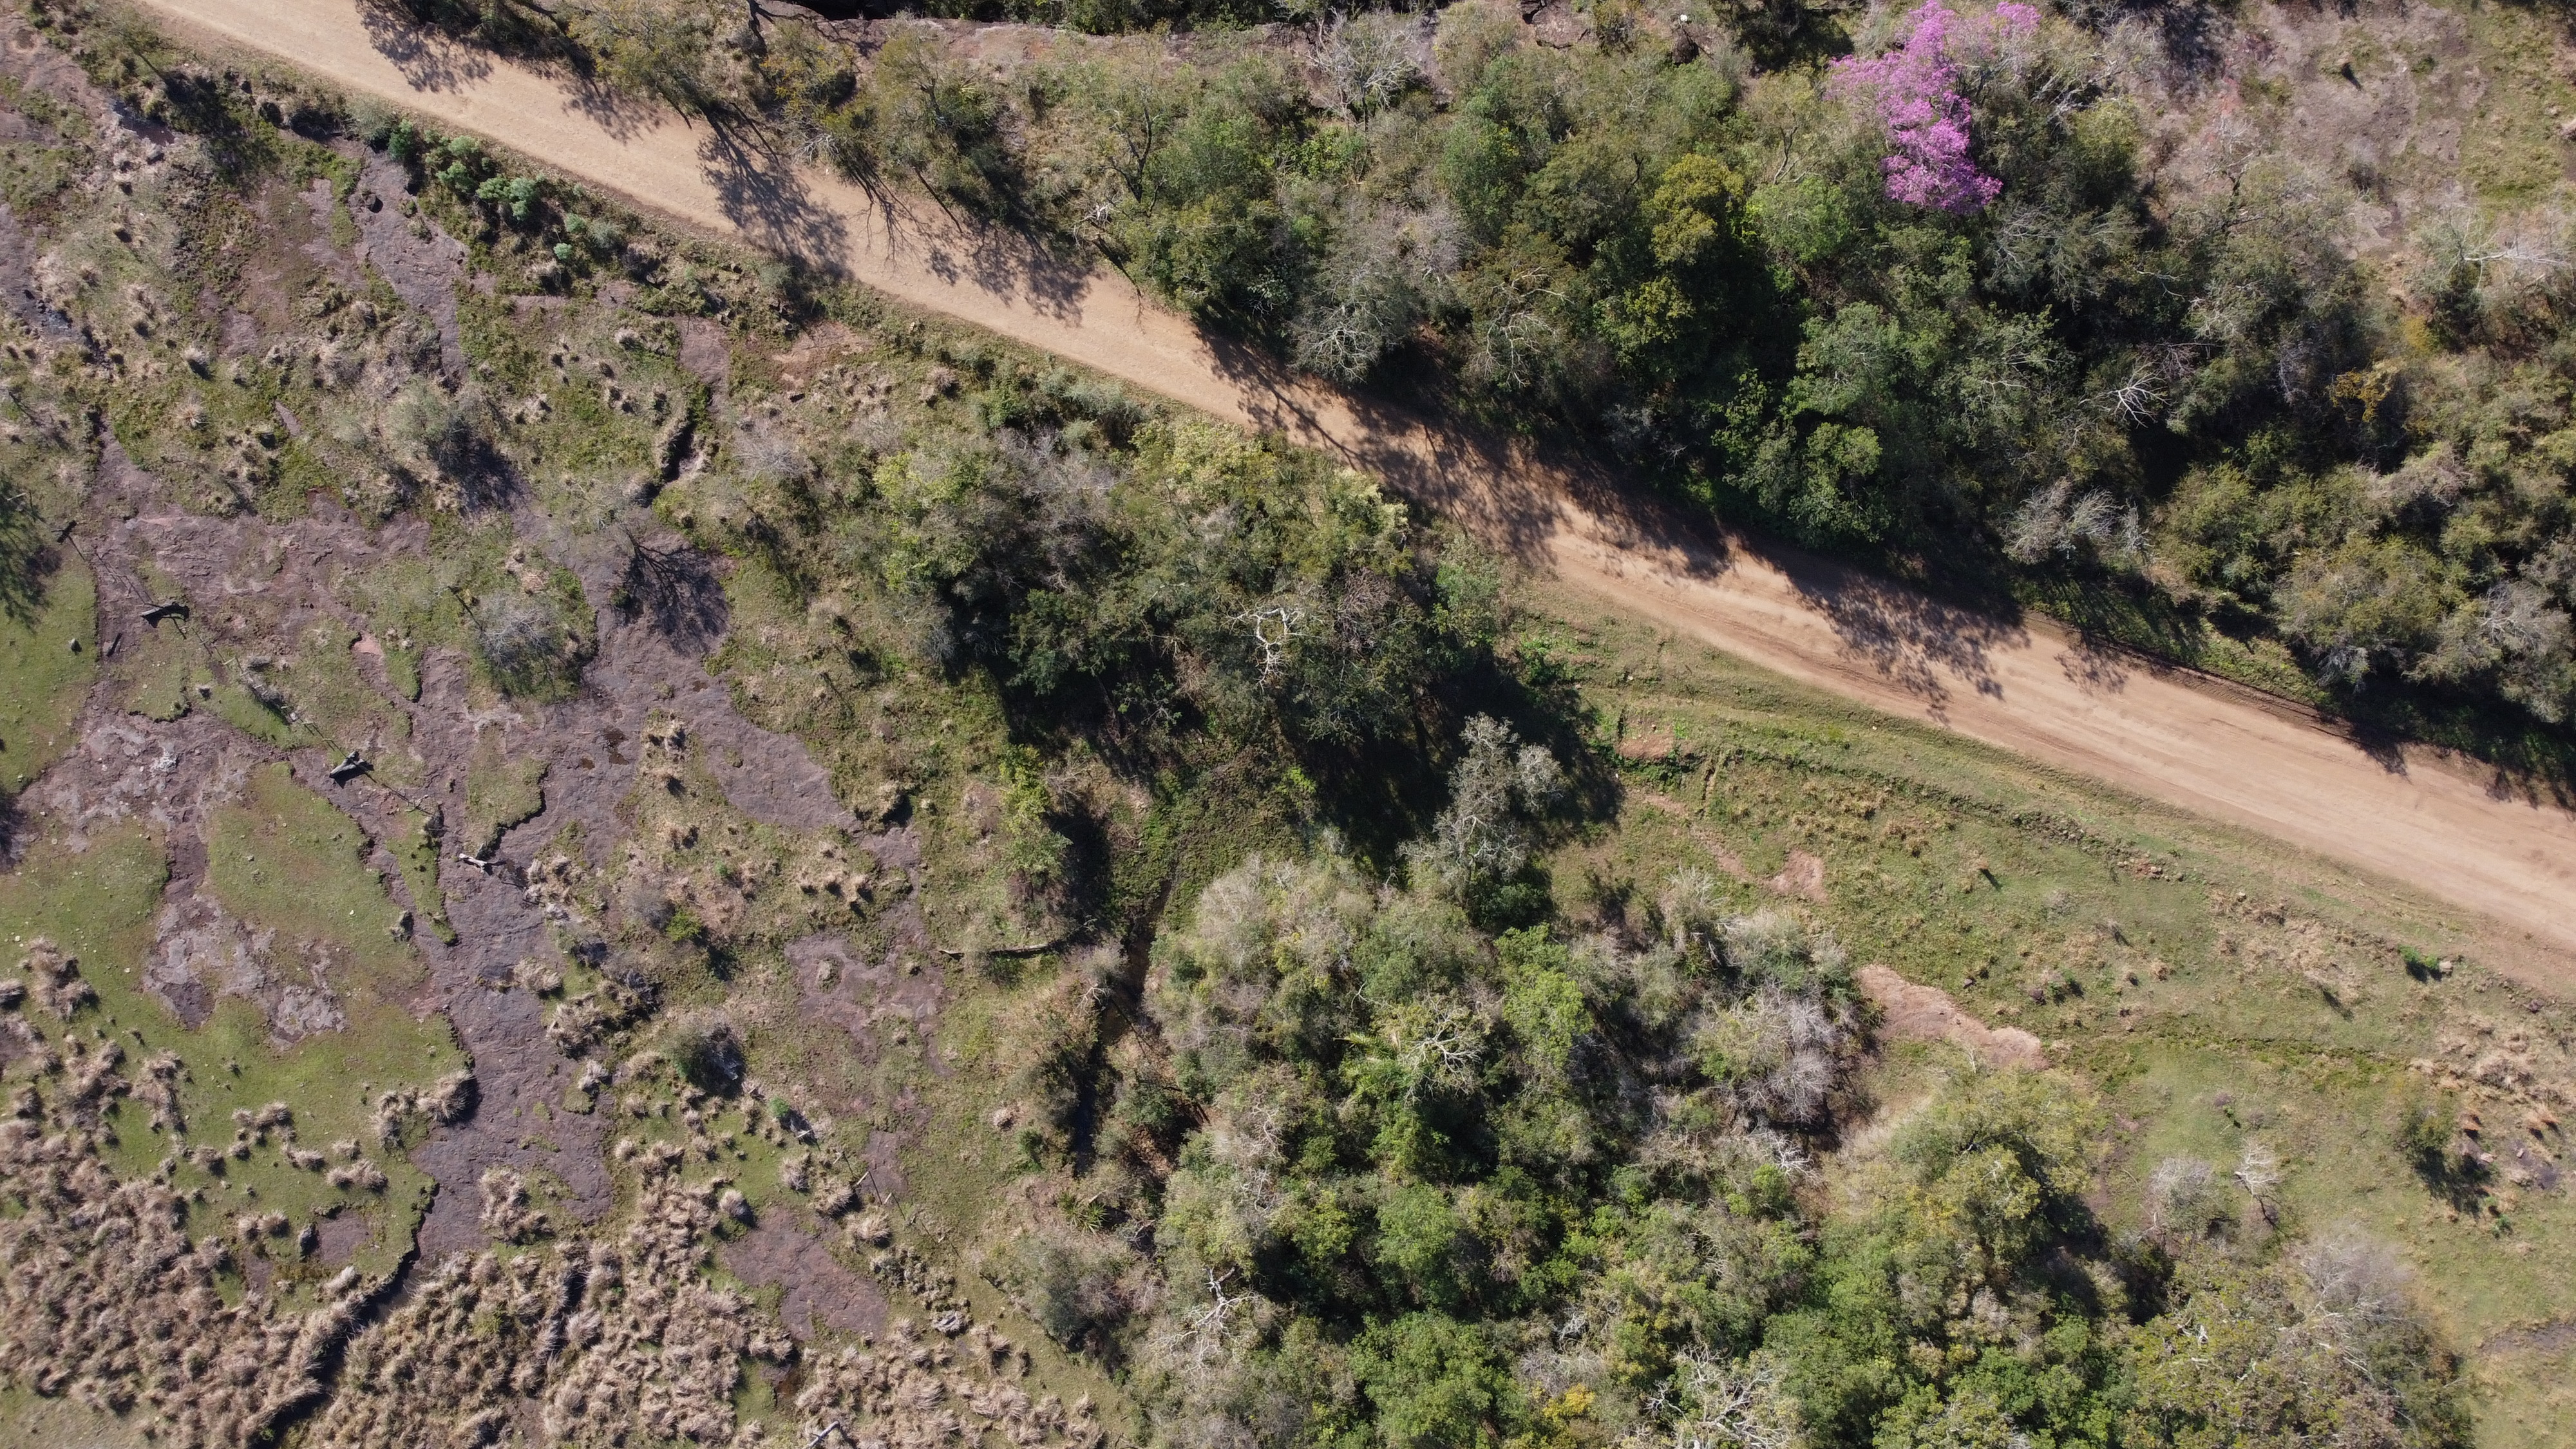
\includegraphics[width=\textwidth]{Imagenes/street.jpg}
     \hfill
     \caption{Escena capturada con pocos árboles}
    \label{calle}
\end{figure}

\begin{figure}[H]
    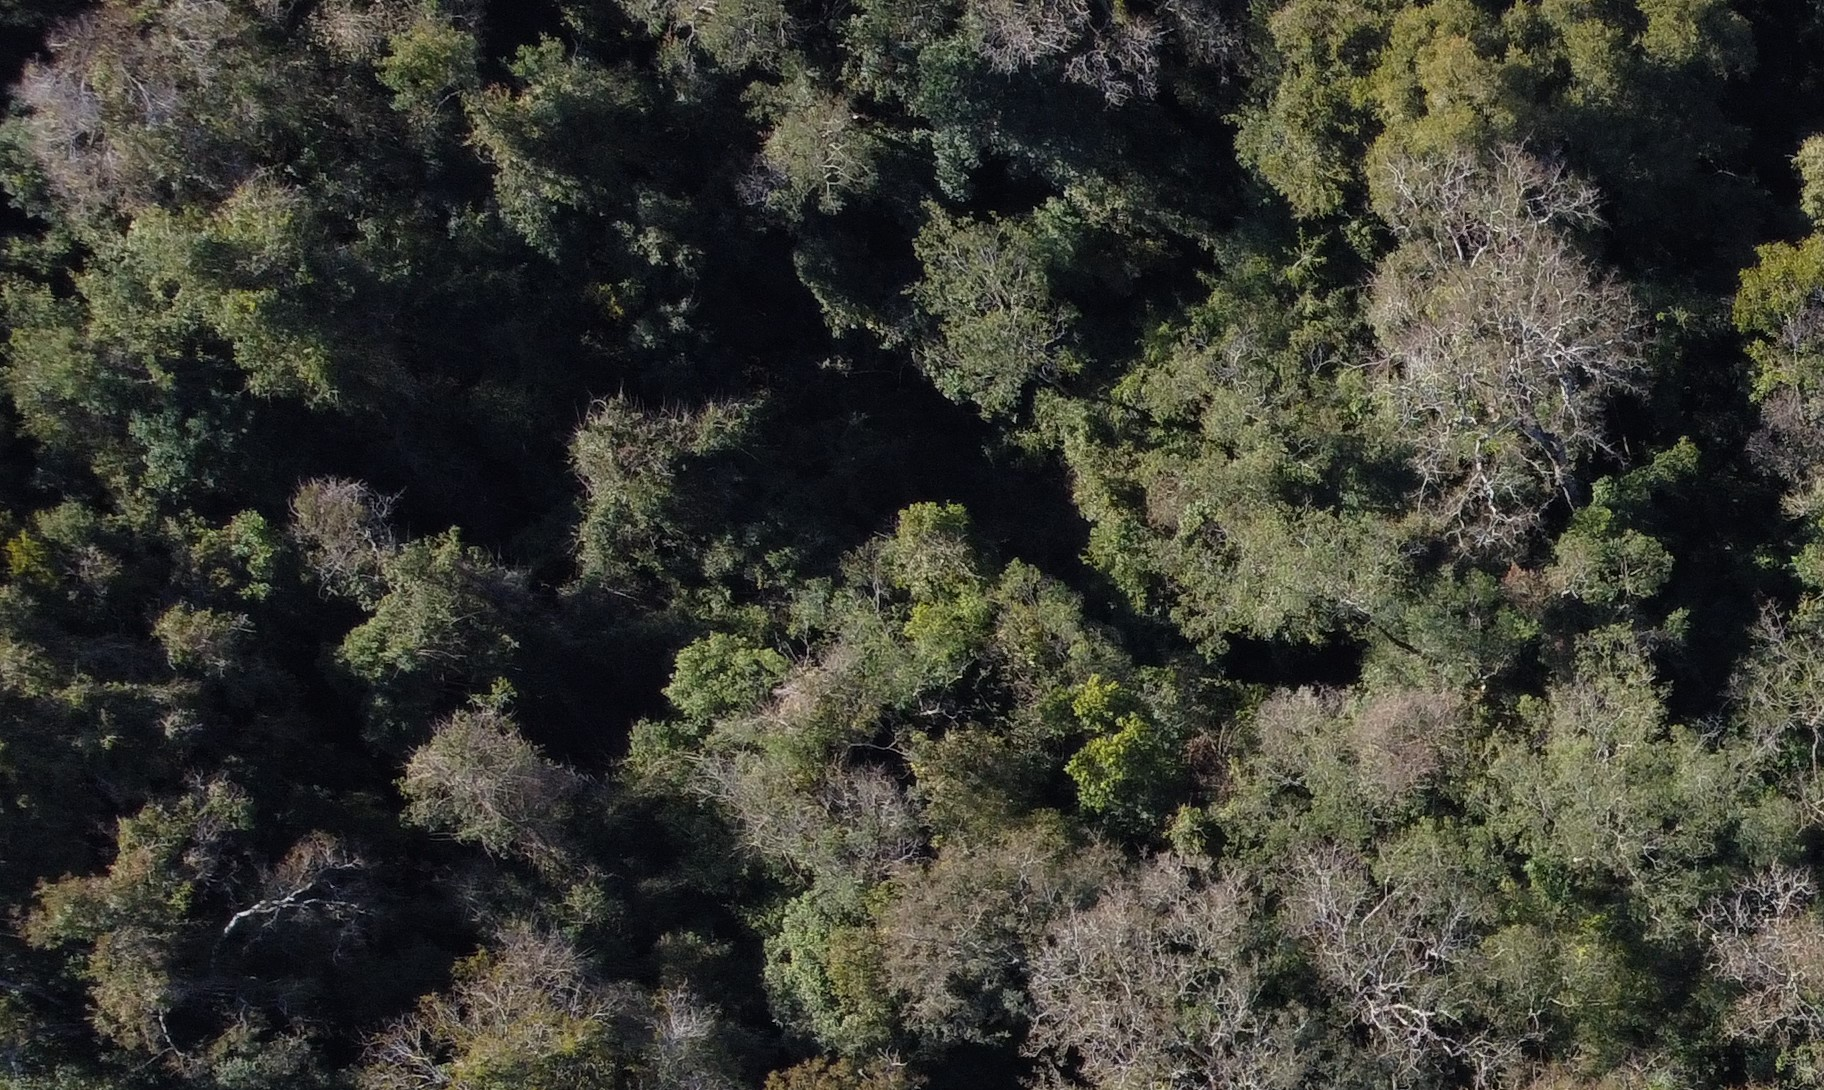
\includegraphics[width=\textwidth]{Imagenes/dense canopy.jpg}
     \hfill
     \caption{Escena capturada con dosel tupido}
    \label{tupido}
\end{figure}


\begin{figure}[H]
    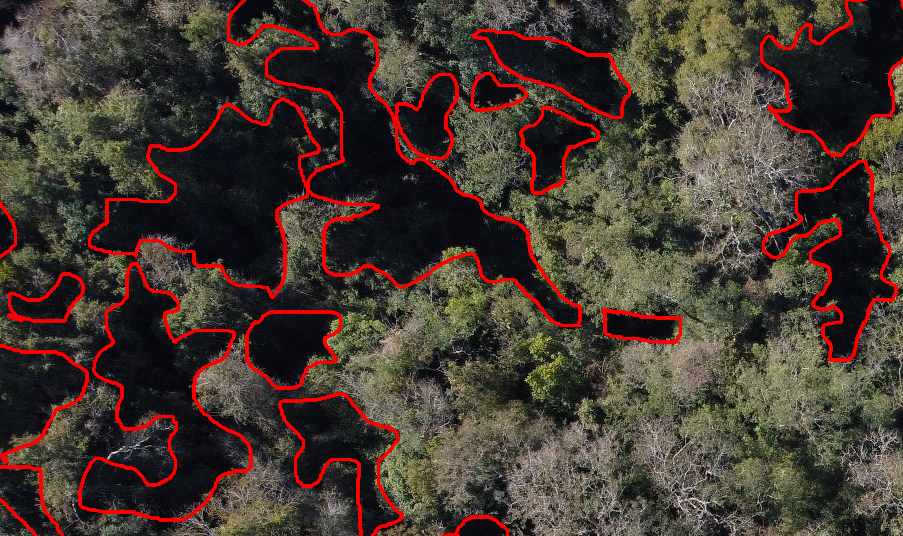
\includegraphics[width=\textwidth]{Imagenes/contours.png}
     \hfill
     \caption{Contornos de sombras en dosel tupido}
    \label{contorno1}
\end{figure}

\begin{figure}[H]
    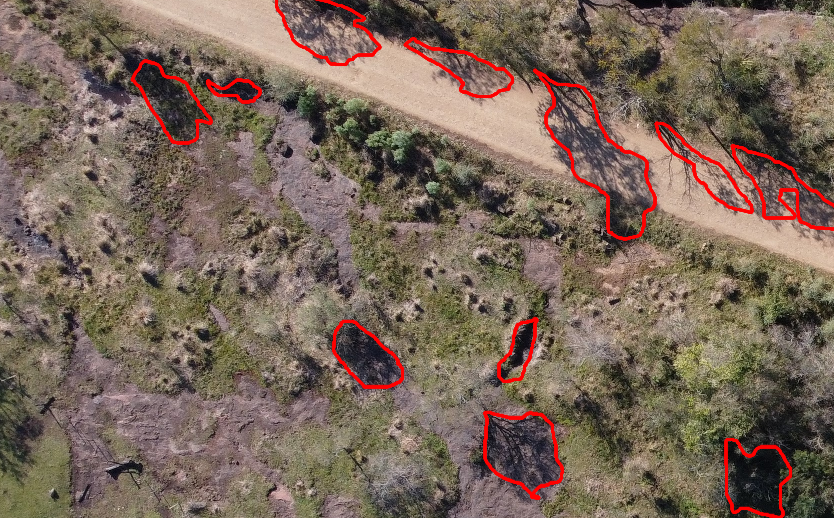
\includegraphics[width=\textwidth]{Imagenes/contours2.png}
     \hfill
     \caption{Contorno de sombras en imagen con pocos árboles}
    \label{contorno2}
\end{figure}

\begin{figure}[H]
     
         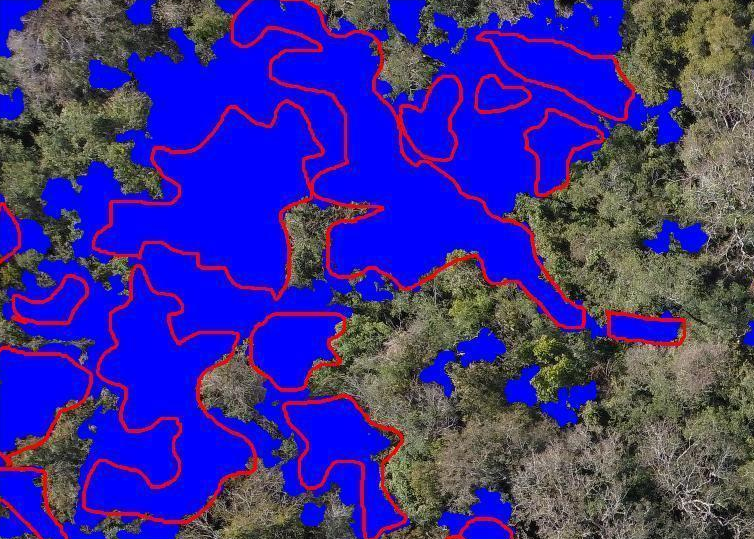
\includegraphics[width=\textwidth]{Imagenes/superposition of masks.png}
         \caption{Superposición de máscaras automática (color azul) y manual (contorno rojo), percentil 60º}
         \label{p60}
\end{figure}
     \hfill
     
\begin{figure}[H]
         
         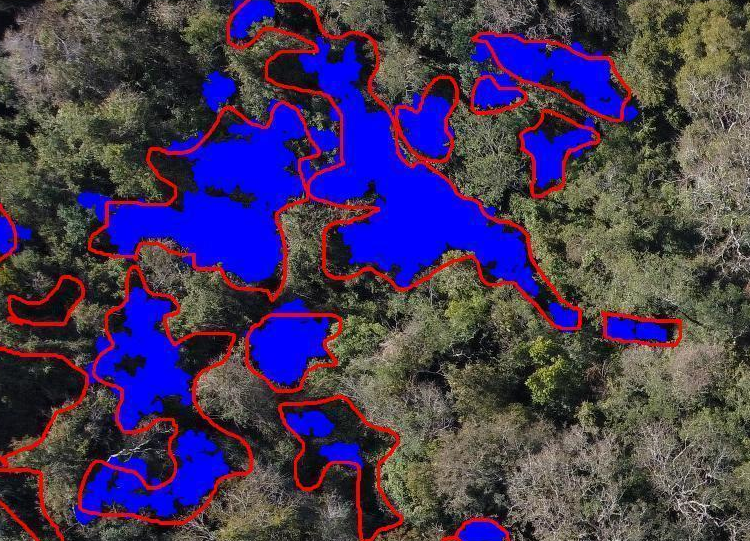
\includegraphics[width=\textwidth]{Imagenes/superposition of masks 2.png}
         \caption{Superposición de máscaras automática (color azul) y manual (contorno rojo), percentil 85º}
         \label{p85}
\end{figure}

\begin{figure}[H]
    
    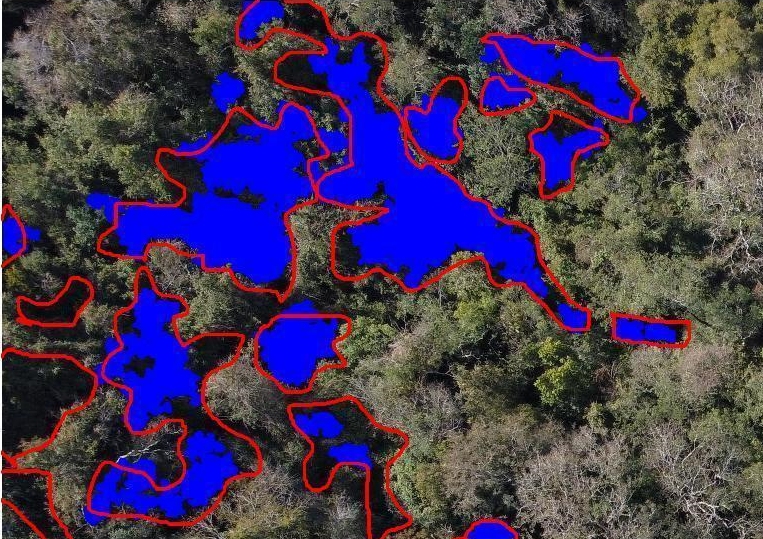
\includegraphics[width=\textwidth]{Imagenes/blue minus red 85.png}
     \hfill
     \caption{Superposición de máscaras automática (color azul) y manual (contorno rojo), percentil 85\textpsi\textsubscript{BR}}
    \label{azulrojo}
 \end{figure}

 \begin{figure}[H]
    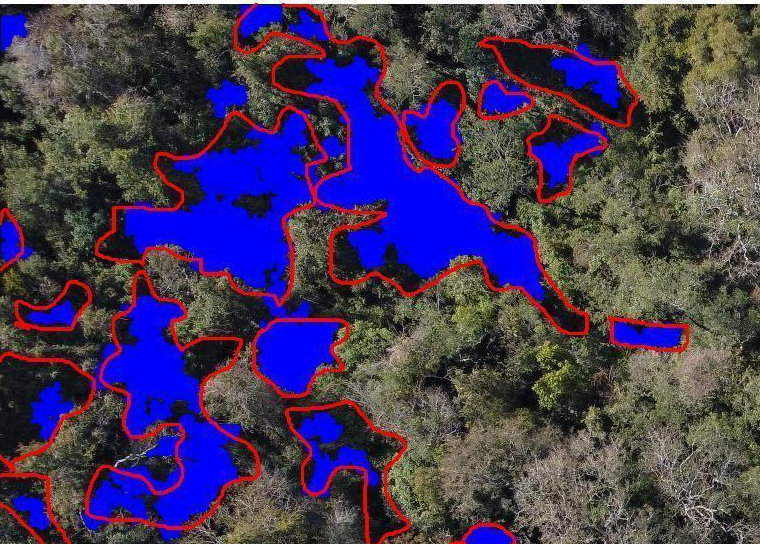
\includegraphics[width=\textwidth]{Imagenes/blue minus green 85.png}
     \hfill
     \caption{Superposición de máscaras automática y manual \textpsi\textsubscript{BG}}
    \label{azulverde}
 \end{figure}

 \begin{figure}[H]
    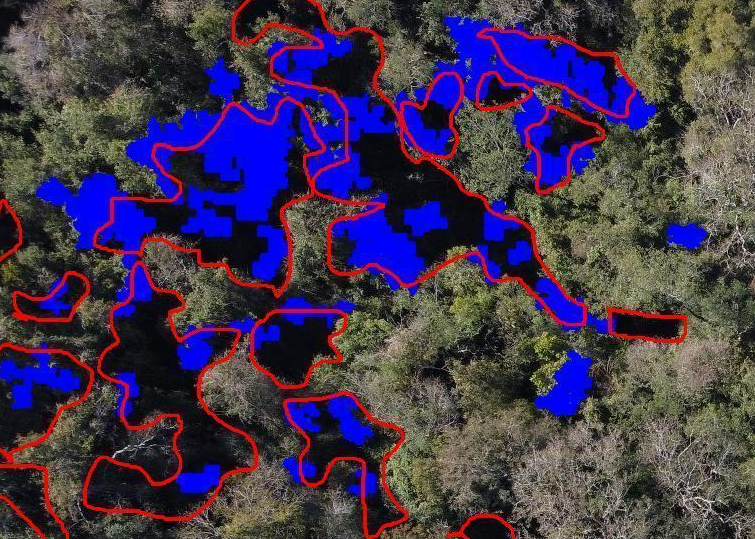
\includegraphics[width=\textwidth]{Imagenes/green minus red 85.png}
     \hfill
     \caption{Superposición de máscaras automática y manual \textpsi\textsubscript{GR}}
    \label{verderojo}
 
\end{figure}

\begin{figure}[H]
    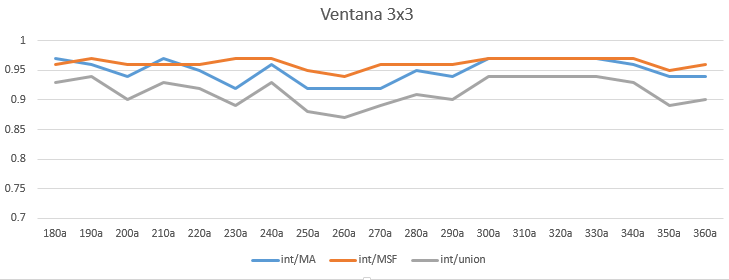
\includegraphics[width=\textwidth]{Imagenes/filter 3x3.png}
     \hfill
     \caption{Filtro 3x3}
    \label{filter3x3}
\end{figure}

\begin{figure}[H]
    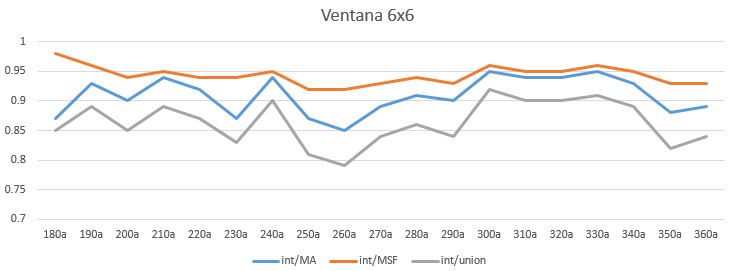
\includegraphics[width=\textwidth]{Imagenes/filter 6x6.png}
     \hfill
     \caption{6x6}
    \label{filter6x6}
\end{figure}

\begin{figure}[H]
    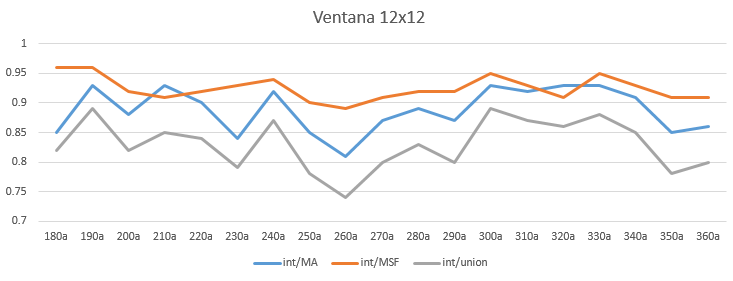
\includegraphics[width=\textwidth]{Imagenes/filter 12x12.png}
     \hfill
     \caption{12x12}
    \label{filter12x12}
\end{figure}
%%%%%%%%%%%%%%%%%%%%%%%%%%%%%%%%%%%%%%%%%%%%%%%%%%%%%%%%%%%%%%%%%%%%%%%%%


%%%%%%%%%%%%%%%%%%%%%%%%%%%%%%%%%%%%%%%%%%%%%%%%%%%%%%%%%%%%%%%%%%%%5

\begin{figure}[H]
    \centering
  \begin{subfigure}[b]{\textwidth}
    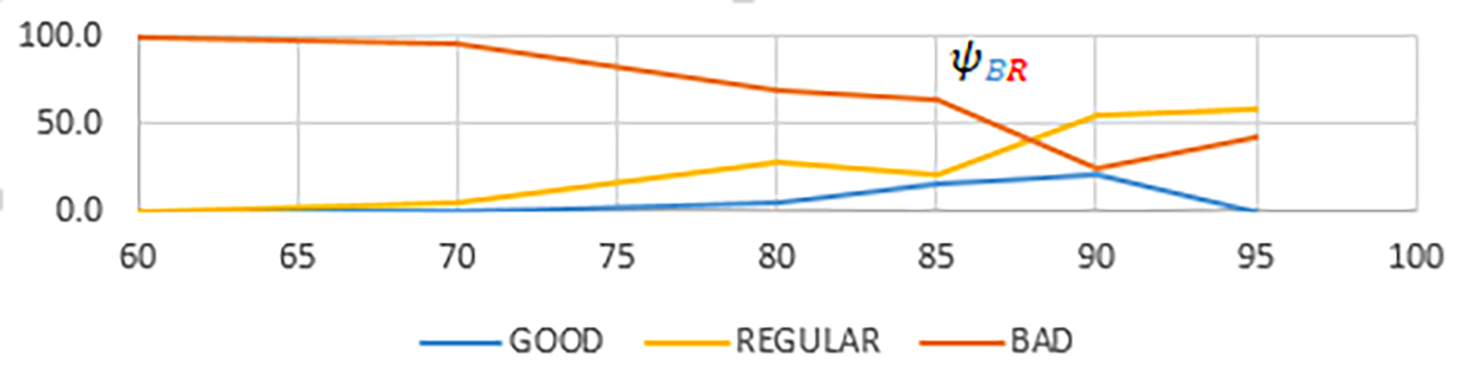
\includegraphics[width=\textwidth]{Imagenes/psiBR.png}
     \hfill
     \caption{Índice $\Psi_{BR}$}
    \label{psiazulrojo}
 \end{subfigure}

 \begin{subfigure}[b]{\textwidth}
    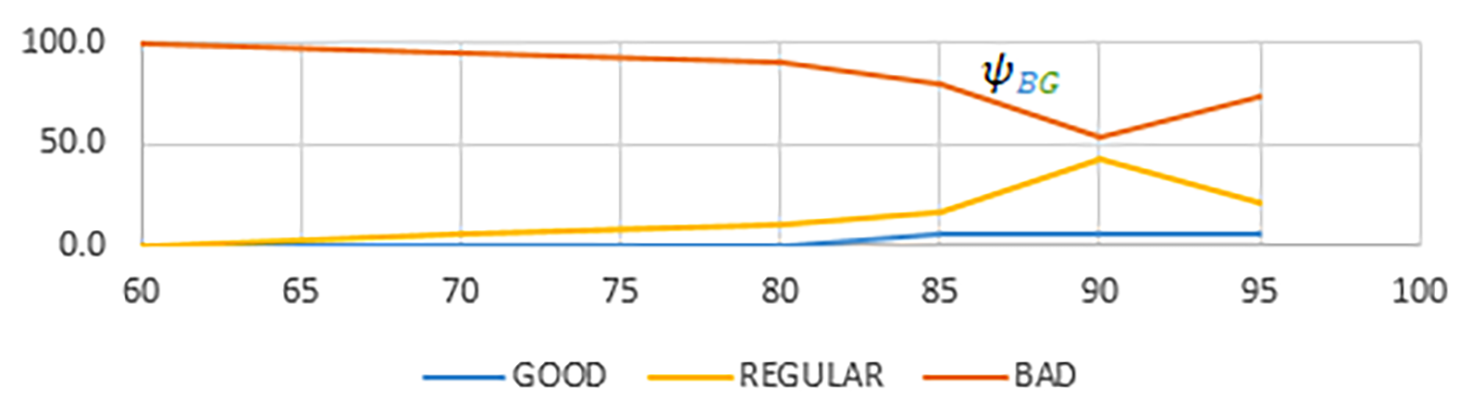
\includegraphics[width=\textwidth]{Imagenes/psiBG.png}
     \hfill
     \caption{Índice $\Psi_{BG}$}
    \label{psiazulverde}
 \end{subfigure}

 \begin{subfigure}[b]{\textwidth}
    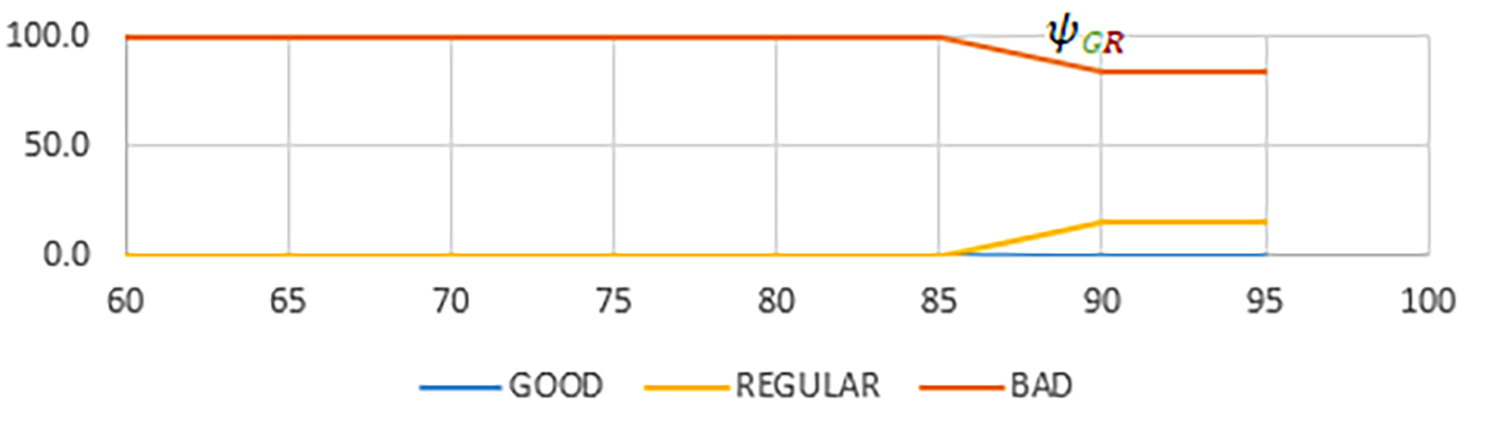
\includegraphics[width=\textwidth]{Imagenes/psiGR.png}
     \hfill
     \caption{Índice $\Psi_{GR}$}
    \label{psiverderojo}
 \end{subfigure}
 \caption{Comparación de máscaras automáticas con manual, para tres casos de índice invariante de color}
        \label{compara_mascara}
\end{figure}